\documentclass{article}
\usepackage{tikz-feynman}

\documentclass{article}
\usepackage{tikz-feynman}

\begin{document}
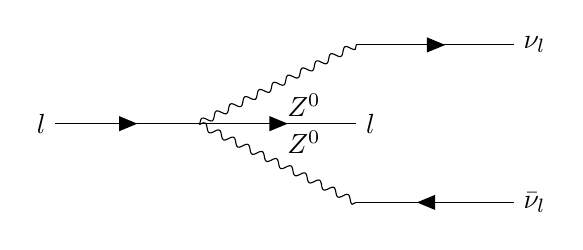
\begin{tikzpicture}
\begin{feynman}
  \vertex (i1) {\(l\)};
  \vertex[right=2cm of i1] (a);
  \vertex[right=2cm of a] (f1) {\(l\)};
  \vertex[above right=1cm and 2cm of a] (v1);
  \vertex[below right=1cm and 2cm of a] (v2);
  \vertex[right=2cm of v1] (f2) {\(\nu_l\)};
  \vertex[right=2cm of v2] (f3) {\(\bar{\nu}_l\)};
  \diagram* {
    (i1) -- [fermion] (a) -- [fermion] (f1),
    (a) -- [boson, edge label'=\(Z^0\)] (v1),
    (v1) -- [fermion] (f2),
    (a) -- [boson, edge label=\(Z^0\)] (v2),
    (v2) -- [anti fermion] (f3),
  };
\end{feynman}
\end{tikzpicture}
\end{document}